% !TEX root = ../thesis-example.tex
%
\chapter{Patterns of segregation}
\label{sec:concepts}

\begin{flushright}{\slshape    
To understand is to perceive patterns.} \\ \medskip
--- Isaiah Berlin~\cite{Berlin:2013}
\end{flushright}


\bigskip


There are many different ways in which a spatial pattern can deviate from its
randomised. This is why we have to further investigate and understand
residential segregation, one needs to develop further measures -- that will
eventually fit in one of the previously mentionned dimensions. The different
dimensions of segregation then correspond to particular aspects of how a
multi-dimensional pattern can deviate from the corresponding unsegregated city.
In this chapter, we will try to quantify these patterns in a way that makes
sense, and is useful to understand the phenomenon of segregation. To do so, it
is always useful to explore the existing literature and look at the difficulties
that have been encountered and mentionned by previous authors.

First, several difficulties are tied to the existence of several categories in
the underlying data. Historically, measurements of racial segregation were
limited to measures between $2$ population groups. However, most measures
generalise poorly to a situation with many groups, and the others do not
necessarily have a clear interpretation~\cite{Reardon:2002}. Worse, in the case
of groups based on a continuum (such as income), the thresholds chosen to define
classes are usually arbitrary~\cite{Jargowsky:1996}. We propose in the following
to solve this issue by defining classes in a unambiguous and non-arbitrary way
through their pattern of spatial interaction. Applied to the distribution of
income categories in US cities, we find $3$ emergent categories, which are
naturally intepreted as the lower-, middle- and higher-income classes. 

Second, most authors systematically design a single index of segregation for
territories that can be very large, up to thousands of square
kilometers~\cite{Apparicio:2000}. In order to mitigate segregation, a more
local, spatial information is however needed: local authorities need to locate
where the poorest and richest concentrate if they want to design efficient
policies to curb, or compensate for, the existing segregation. In other words,
we need to provide a clear {\it spatial} information on the pattern of
segregation. 

The lack of clear spatial characterization of the distribution of individuals is
not tied to the problem of segregation in particular, but pertains to the field
of spatial statistics~\cite{Ripley:1981}. Many studies avoided this spatial
problem by considering cities as monocentric and circular, and rely on either an
arbitrary definition of the city center boundaries, or on indices computed as a
function to the distance to the center (whatever this may be). However, most if
not all cities are anistropic, and the large ones, polycentric
(\cite{Louf:2013_polycentric}
and references therein), casting some doubt about the application of the
monocentric city picture. Many empirical studies and models in economics aim to
explain the difference between central cities and suburbs \cite{Glaeser:2008,
Brueckner:1999}. Yet, the sole stylized fact upon which they rely -- city centers
tend to be poorer than suburbs (in the US) -- lacks a solid empirical
basis.\\

Data present themselves as the population sorted in different categories, and in
different tracts.

In the following, we will purport to answer the following question, solve the
following difficulties.

\begin{itemize}
    \item How to quantify the presence of the different categories in areal
        units? Can we say whether they are overrepresented or normally
        represented? How can we define neighbourhoods?
    \item How can we quantify the interactions between the different categories?
    \item How to define meaningful classes from the original data?
    \item Do classes tend to leave in geographically coherent areas, or are they
        scattered across the city?
    \item How concentrated are neighbourhoods?
    \item Is there a difference between the city center and the suburbs? How
        shall we quantify this properly?
    \item How to define a meaningful segregation index that generalises easily
        to the many classes situation, and takes the geographical pattern into
        consideration?
\end{itemize}

\section{Presence of categories}
\label{sec:presence_of_categories}

\begin{equation}
    \frac{n_\alpha(t)}{N_\alpha}
\end{equation}


\begin{equation}
    \frac{n_\alpha(t)}{n(t)}
\end{equation}

\subsection{An unbiaised measure: representation}
\label{sub:an_unbiaised_measure_the_representation}

\begin{equation}
    r_alpha(t) = \frac{n_\alpha(t)/n(t)}{N_\alpha/N}
\end{equation}

\section{Measuring the attraction and repulsion of categories}
\label{sec:measuring_the_attraction_and_repulsion_of_categories}

\begin{equation}
    E_{\alpha \beta}(t) = \frac{1}{N_\alpha}
    \sum_{t=1}^T\,n_\alpha(t)\,r_\beta(t) 
\end{equation}

The measure of exposure is symmetric, $E_{\alpha \beta}(t) = E_{\beta \alpha}(t)$

\section{The emergent social classes}
\label{sec:the_emergent_social_classes}


\begin{figure}
    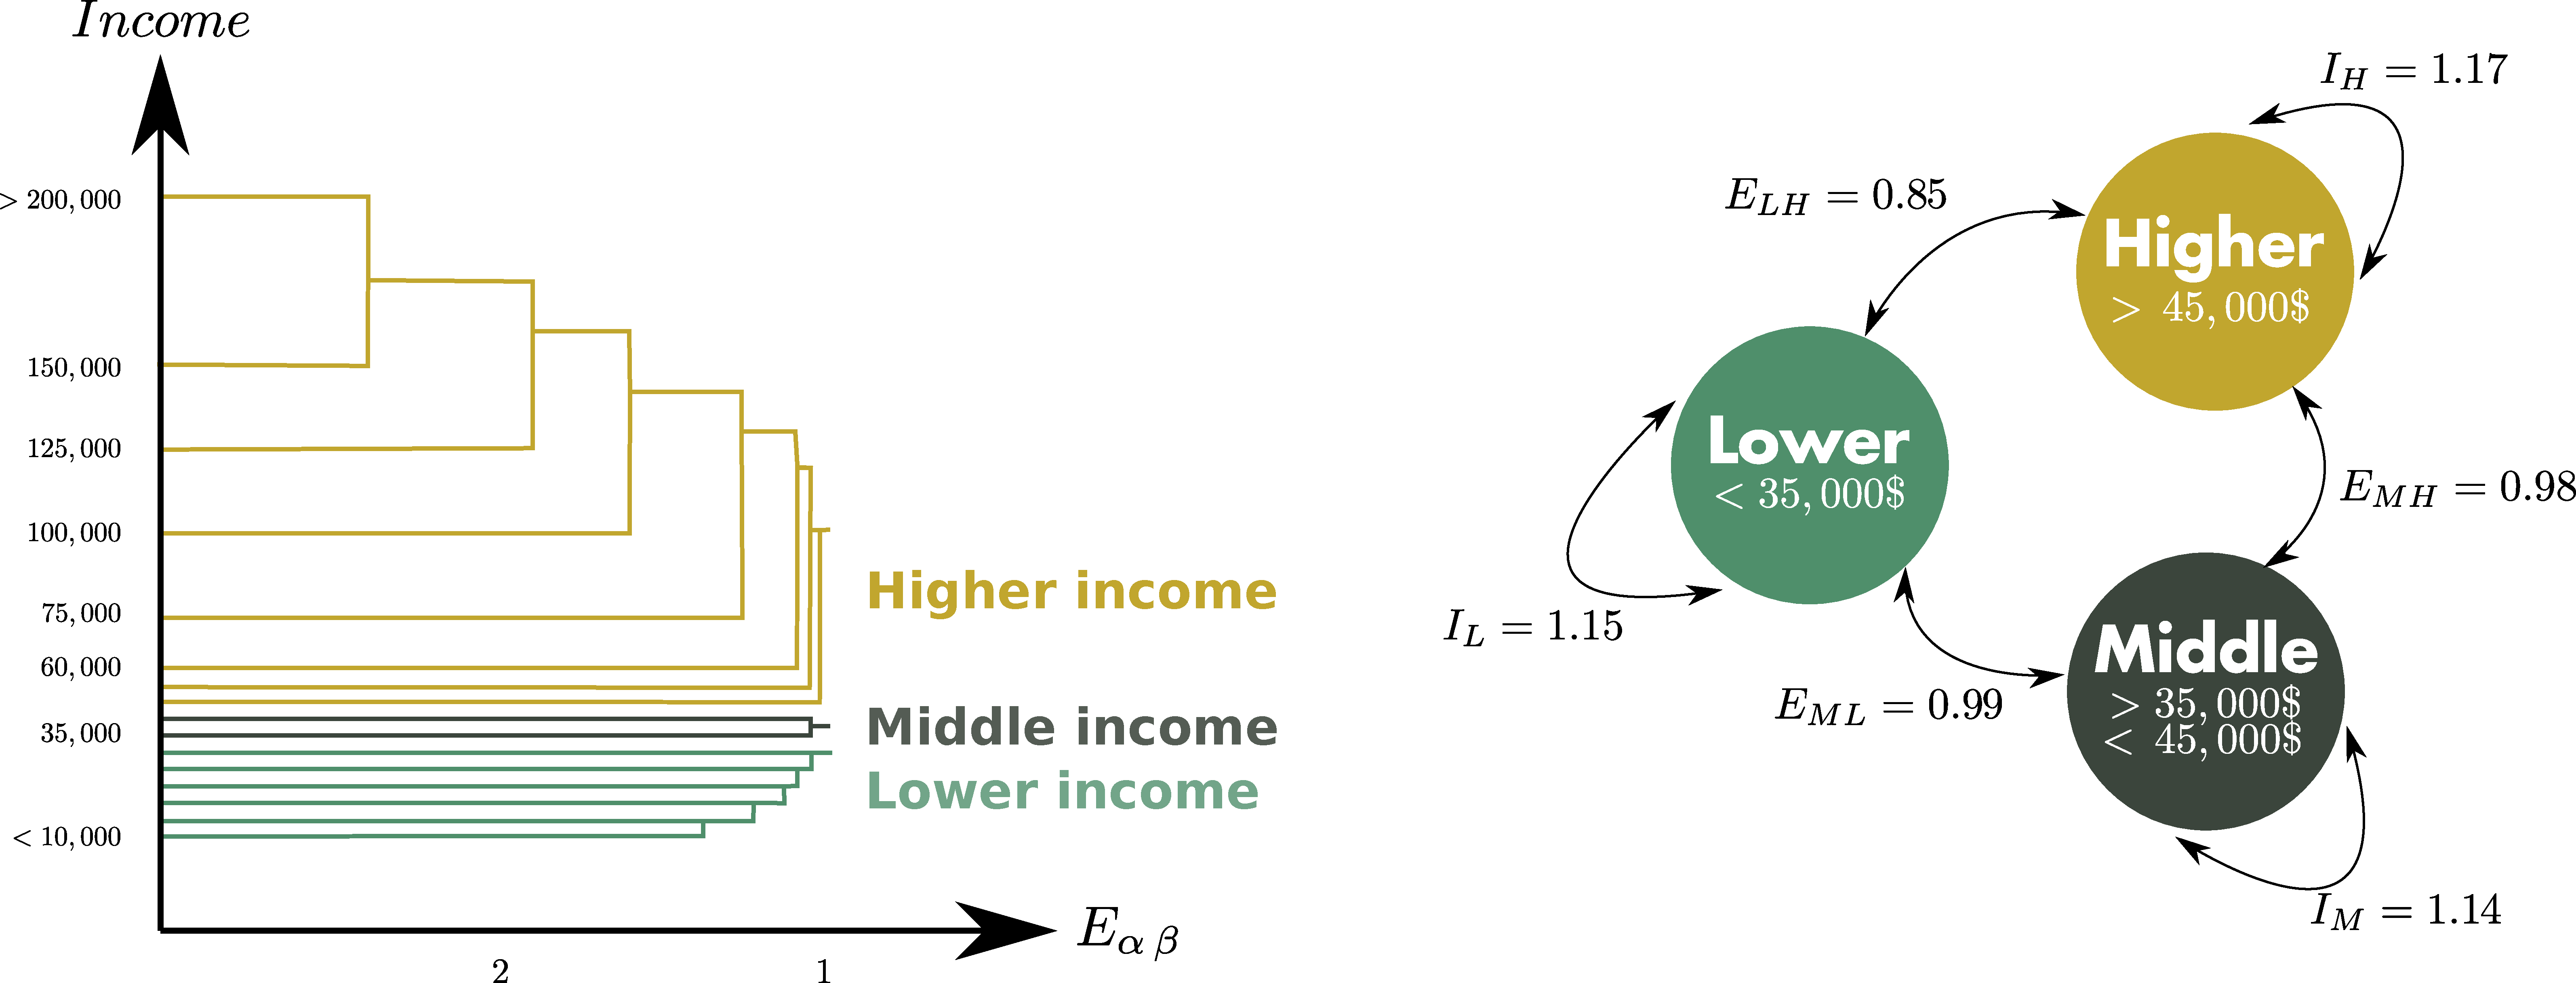
\includegraphics[width=\textwidth]{./gfx/chapter-segregation/figure1.pdf}
    \caption{(a) Alluvial diagram showing the successive aggregations
      of different income categories in the clustering process, and
      the value of the exposure at which the aggregation took
      place. The aggregation stops when there is no pair of category
      for which $E>1$, that is when all classes are at best
      indifferent to one another (see the SI Appendix, section 2 for a more
      detailed description of the algorithm). One can see on this diagram that
      the highest income categories attract one another more (higher values of
      $E_{\alpha \beta}$) than the lowest income categories. (b) The classes that emerge from our
      analysis, and their respective exposure and isolation values. The lower
      and higher income classes repel one another, while the middle
      income class is indifferent to either other classes.  The
      higher-income class is more coherent than the lower-income,
      which is more coherent than the middle-income class, as
      reflected by the isolation coefficient $I$.}
\label{fig:classes_alluvial}
\end{figure}


\begin{figure}[!h]
    \centering
    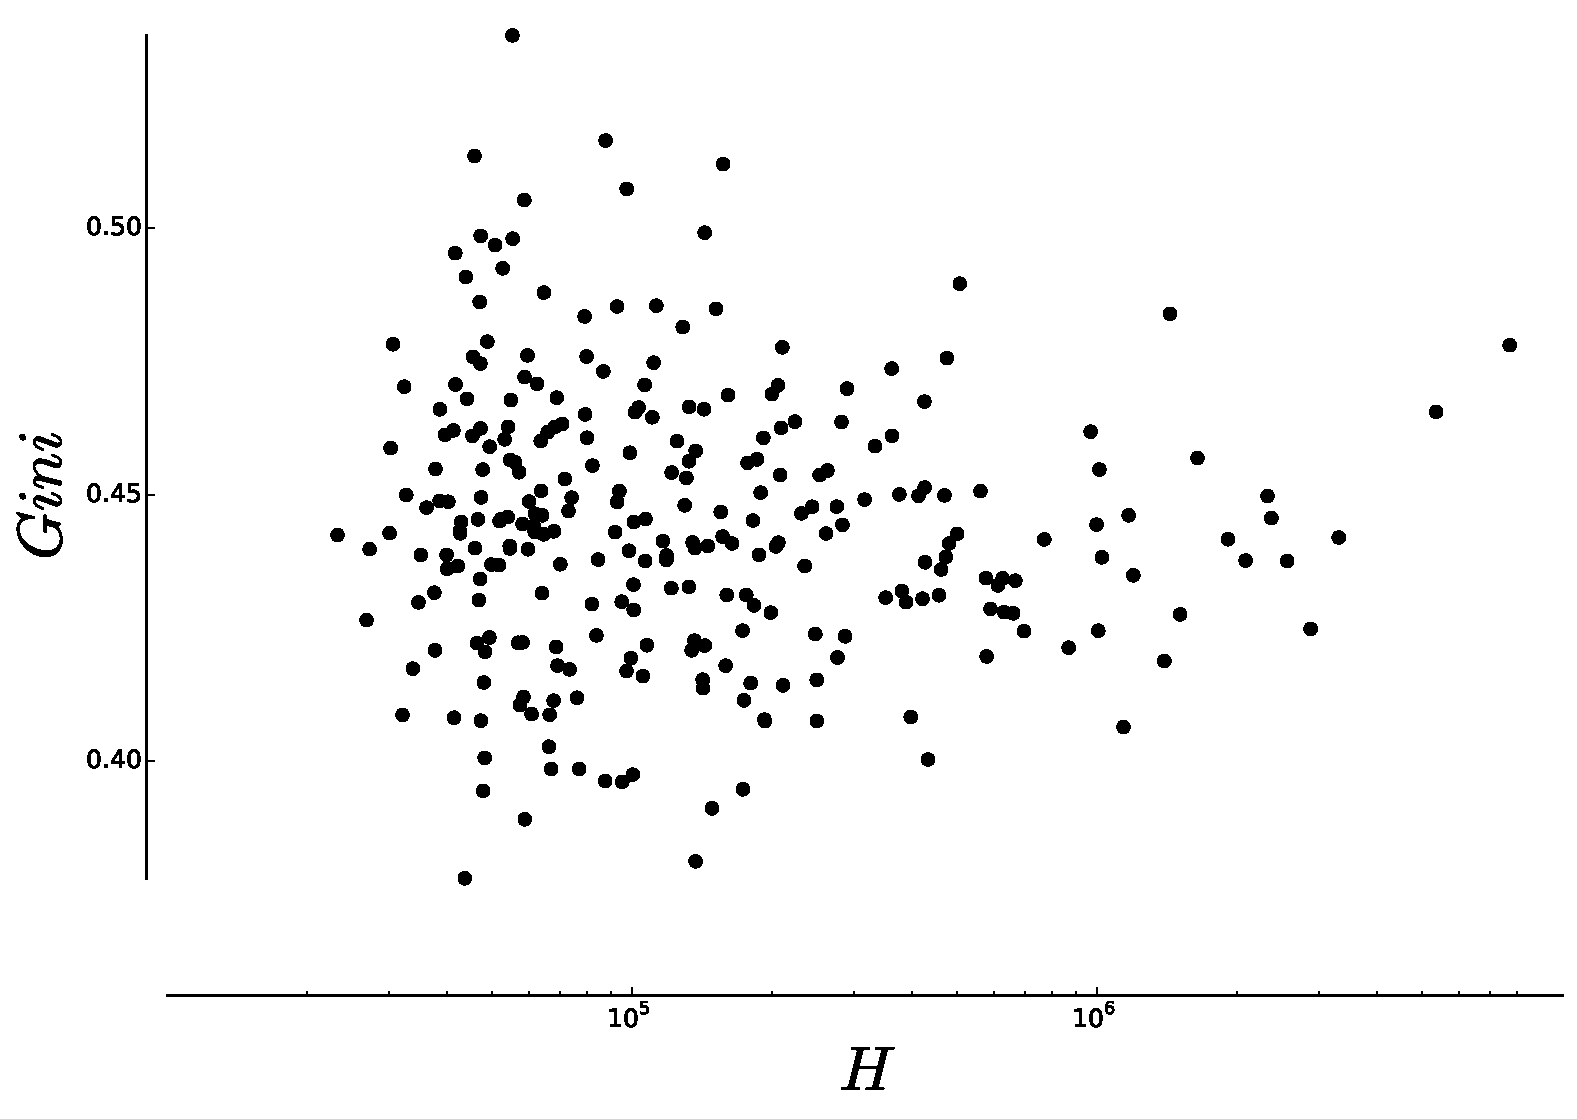
\includegraphics[width=\textwidth]{./gfx/chapter-segregation/gini_income.pdf}
    \caption{Gini coefficient of the income distribution of the $280$ MSA in
    $2000$ versus the number of households in the city. As one can see, there is
no clear relationship.\label{fig:gini}}
\end{figure}

\begin{figure}
    \centering
    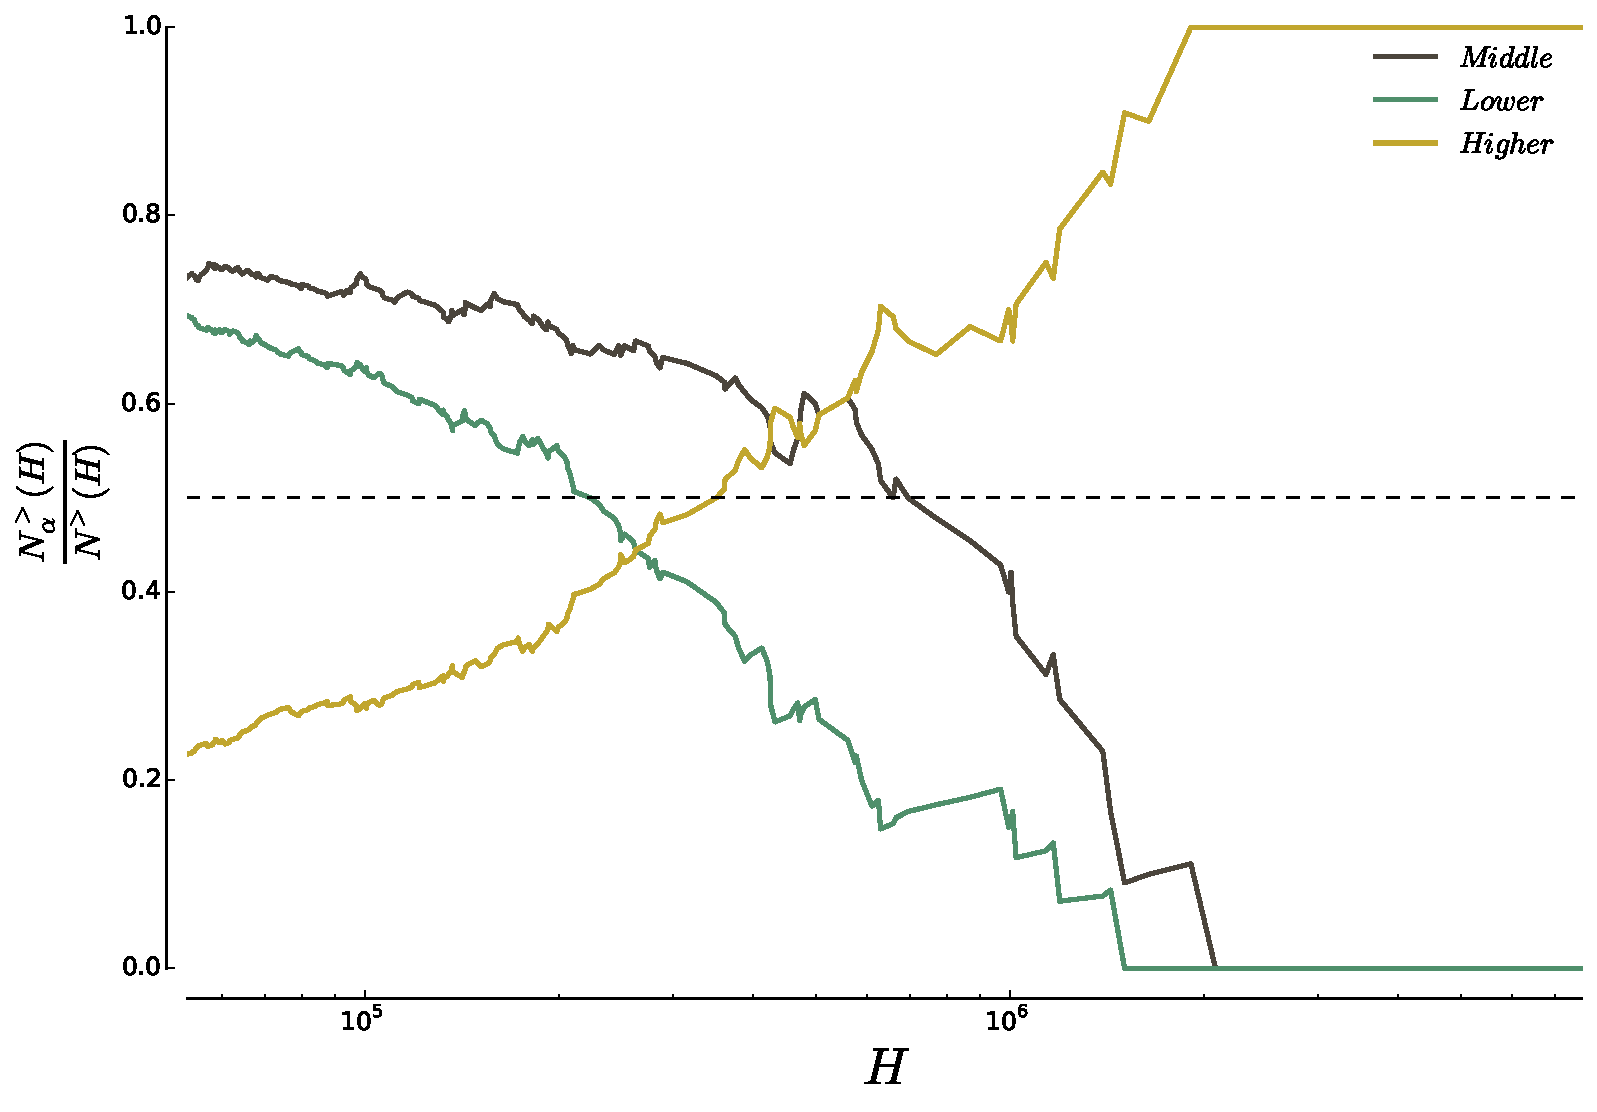
\includegraphics[width=\textwidth]{gfx/chapter-segregation/figure3.pdf}
    \caption{Proportion of cities in which the different classes are
    overrepresented, as a function of the total population of the city. One can
    clearly see that as cities get larger rich people will
    be overrepresented and poor people underrepresented (compared to national
    levels). \label{fig:inter-urban_representation}}
\end{figure}




\section{Neighbourhoods}
\label{sec:neighbourhoods}



\begin{figure}
    \centering
    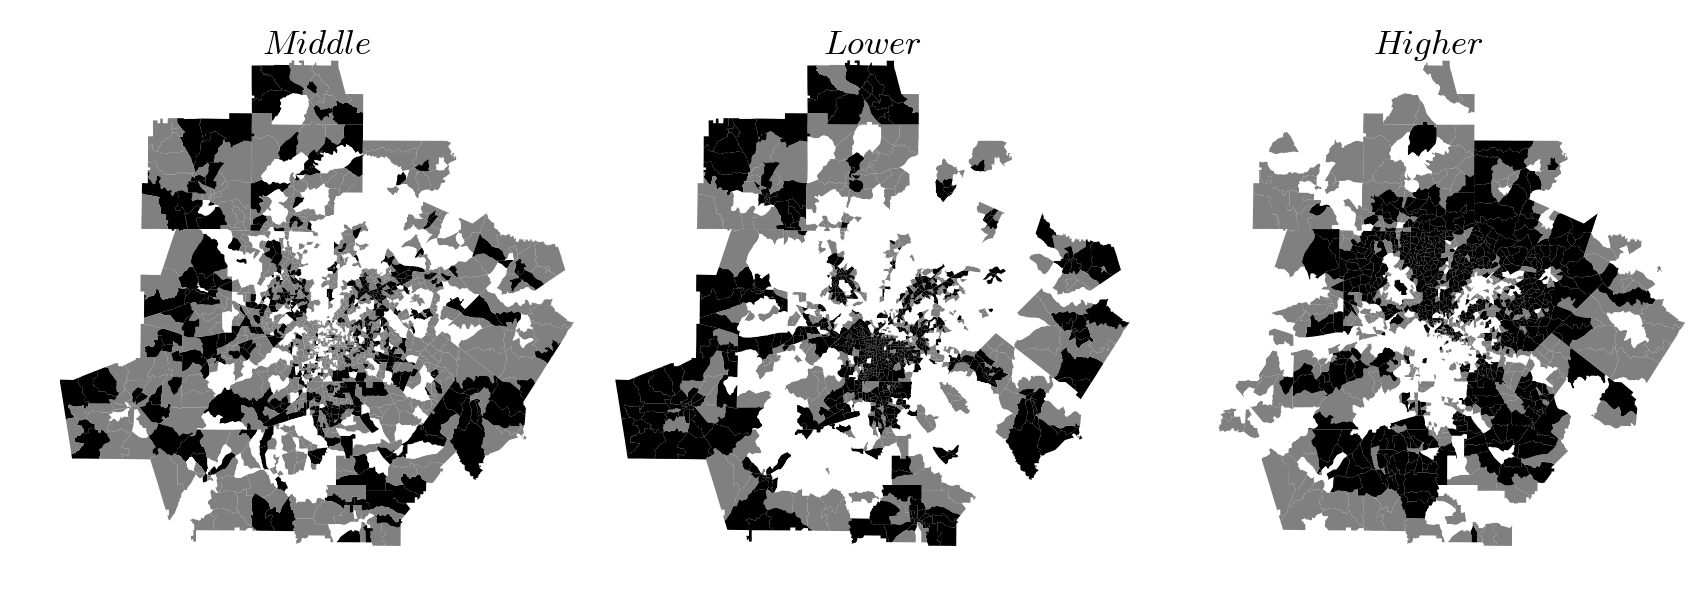
\includegraphics[width=\textwidth]{./gfx/chapter-segregation/figure2.png}
    \caption{The neighbourhoods in Atlanta for the three different
      income category. In black, the tracts where the corresponding
      class is overrepresented, in white where it is
      underrepresented and in grey where its value is
      undistinguishable from the random distribution. All
      MSA defined for the $2000$ Census exhibit a total exclusion between
      lower-income and higher-income
      neighbourhoods: the pictures for lower- and higher-income classes are the
      perfect negative of one another. In contrast, middle-income households
      are scattered across the city and exhibit very little geographical coherence.}
\label{fig:atlanta_neighbourhoods}
\end{figure}


\section{Clustering and concentration}
\label{sec:clustering_and_concentration}



\begin{figure}
    \centering
    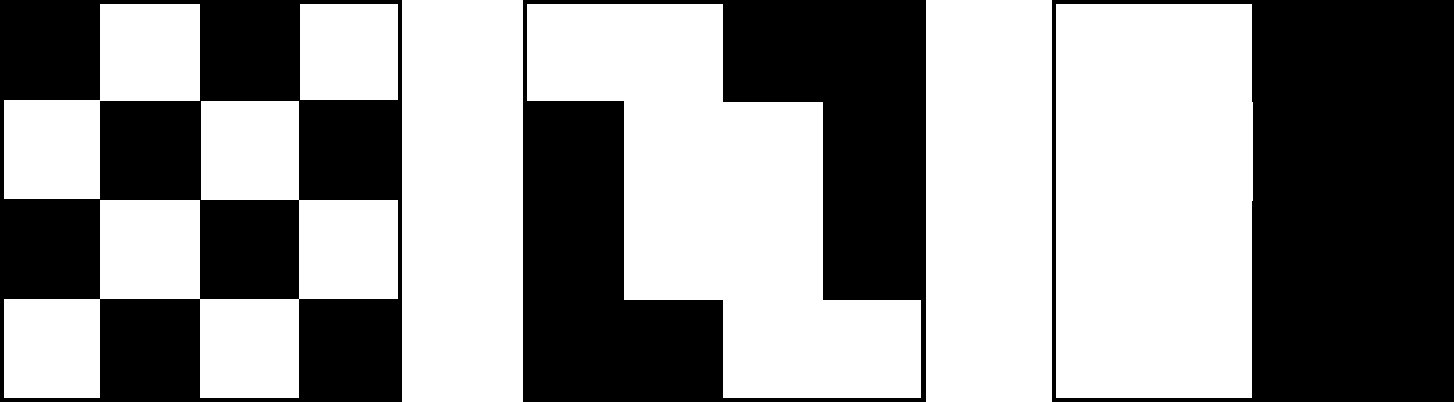
\includegraphics[width=\textwidth]{./gfx/chapter-segregation/figure5.pdf}
    \caption{Three situations that are identical for intra-areal unit measures,
        but that represent different segregation levels. (Left) The checkerboard
        city popularised by White~\cite{White:1983}, corresponding to a
        clustering value of $C=0$ for the black squares. (Middle) An
        intermediate situation between the checkerboard and the divided city,
        corresponding to $C \approx 0.86$.(Right) The divided city, corresponding to
        $C=1$. \label{fig:checkerboard}} 
\end{figure}


\begin{figure} 
    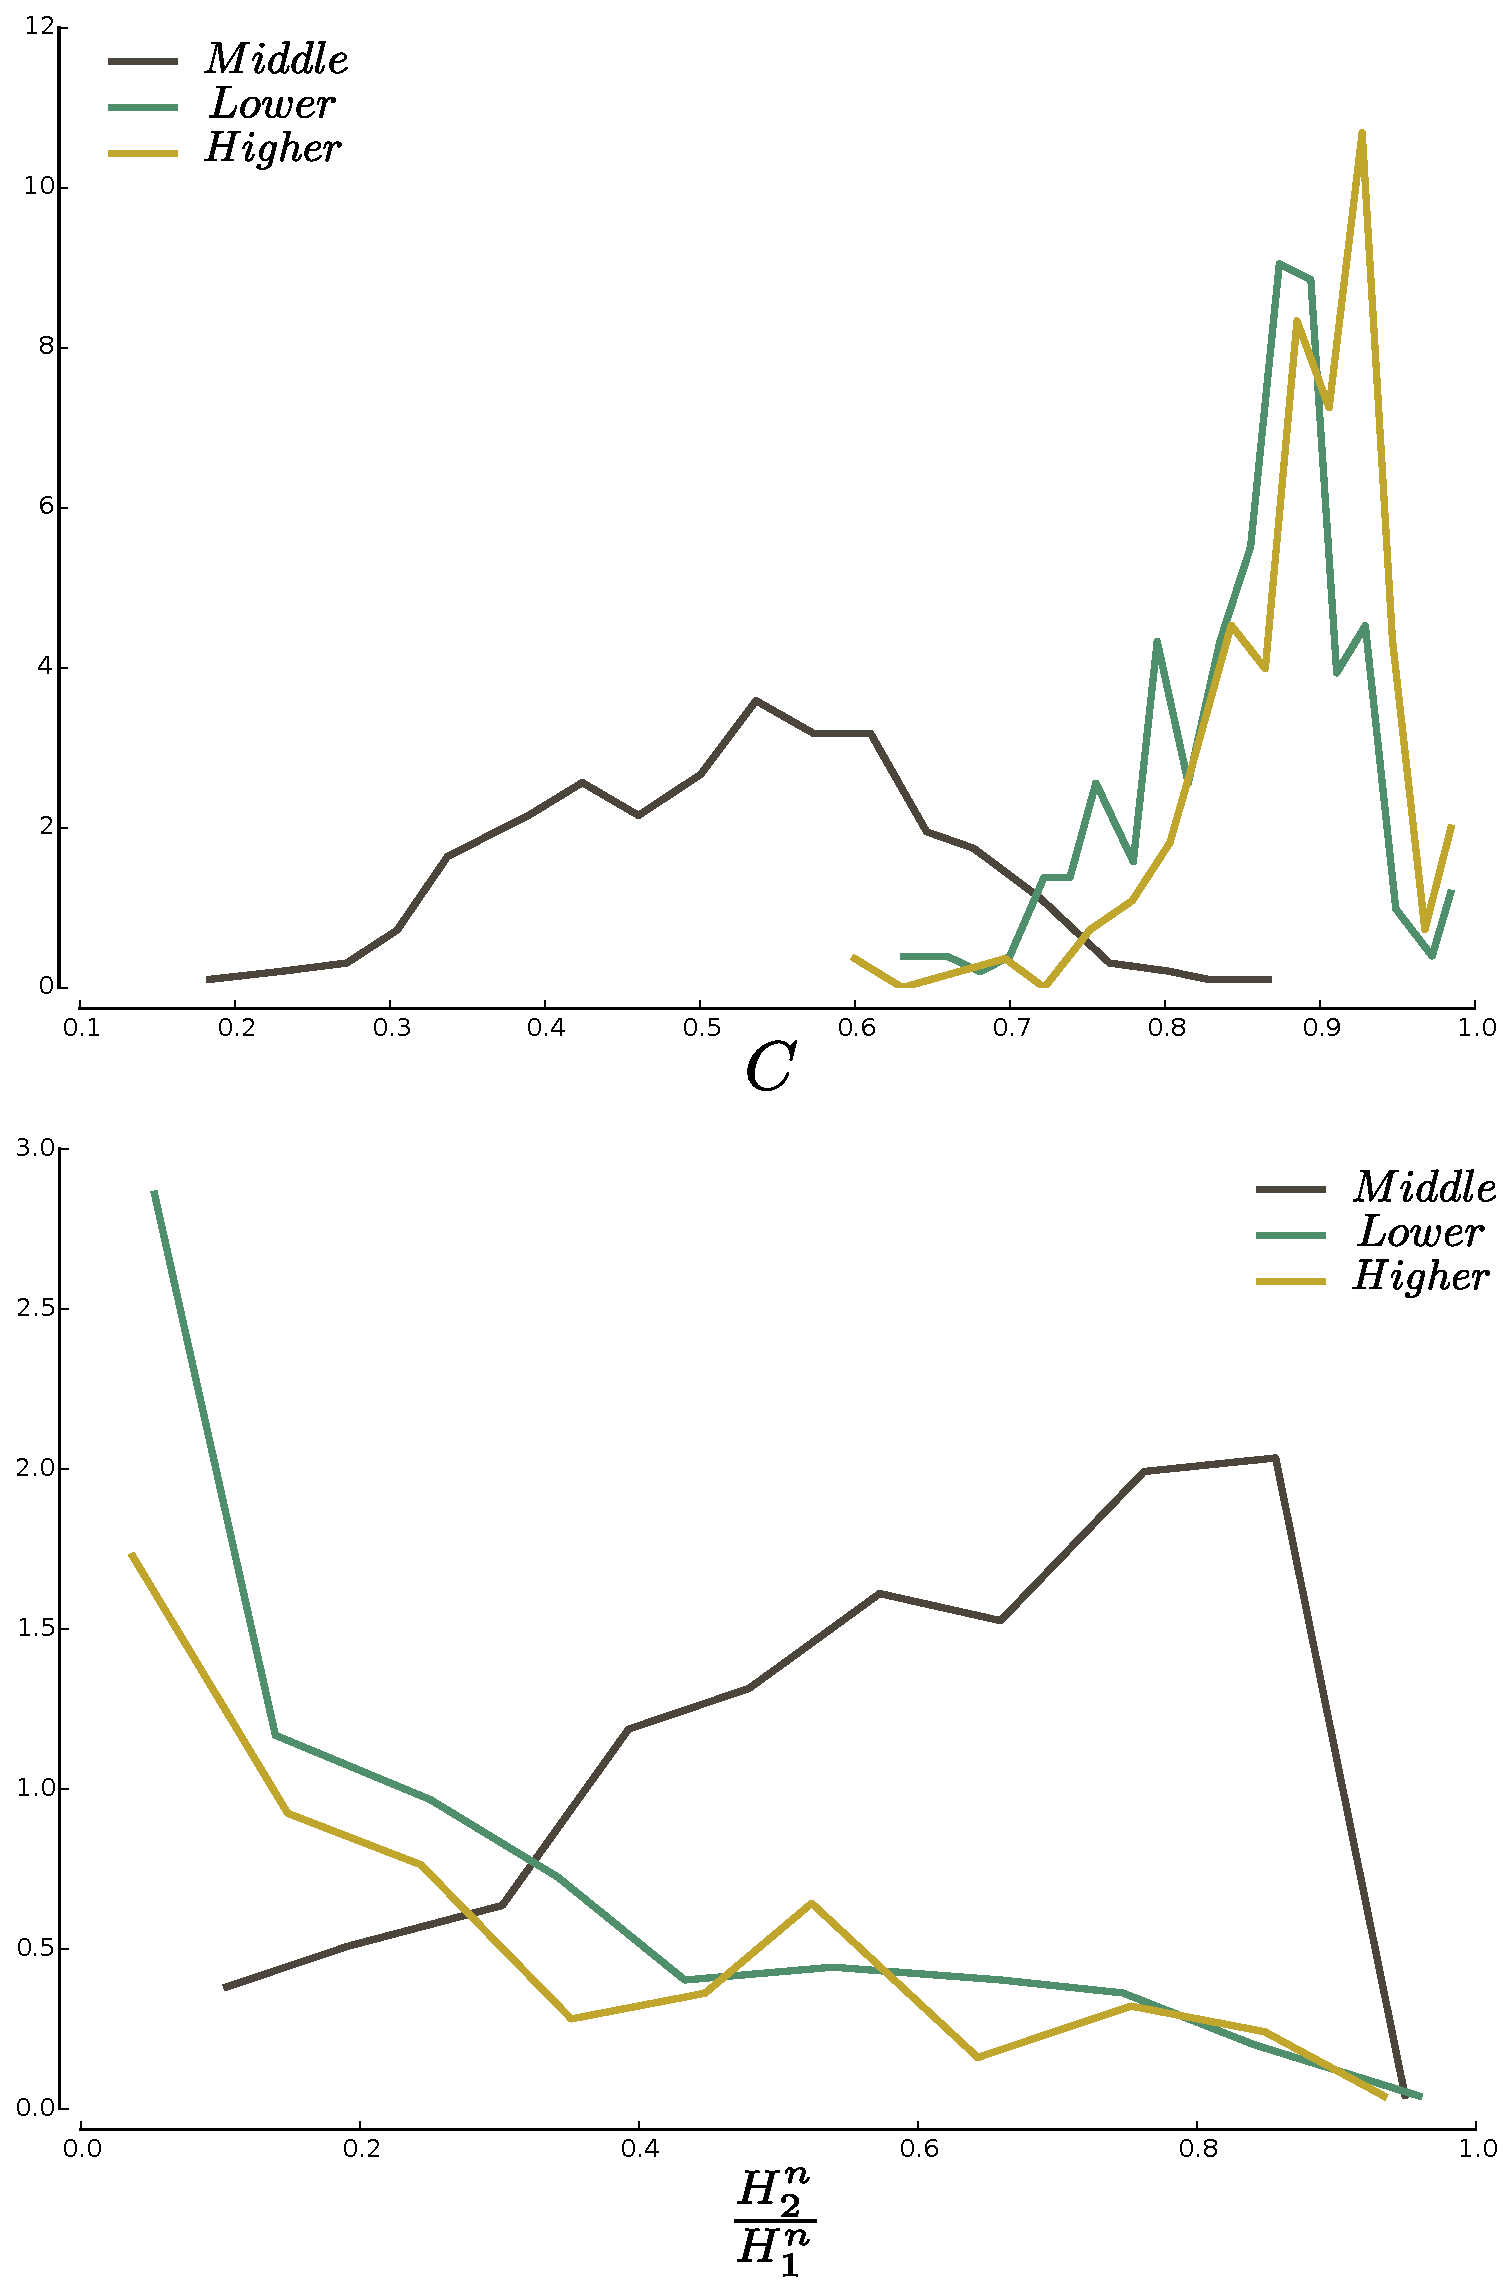
\includegraphics[width=\textwidth]{gfx/chapter-segregation/figure6.pdf}\\
    \caption{(Top) Distribution of the value of the clustering coefficient for
        all cities in our dataset, for the 3 classes. The higher income class
        exhibits the highest level of clustering, with an average of
        $\overline{C} = 0.90$, followed by the lower income class with on
        average $\overline{C} = 0.87$. The Middle income class households are
        significantly less clustered than the previous two, with $\overline{C} =
        0.56$ on average.  (Bottom) Distribution of the ratio of the size of the
        largest and second largest neighbourhoods for each class for all cities in our
        datset. Higher- and lower-income househols tend to concentrate in single
        neighbourhood, with a secondary center that is on average $22\%$ and
        $26\%$ the size of the largest one, respectively. Middle-income
        households tend to be more dispersed, with a secondary neighbourhood that is on
        average $62\%$ of the size of the largest.} \label{fig:clustering} 
\end{figure}


\begin{figure}
    \centering
    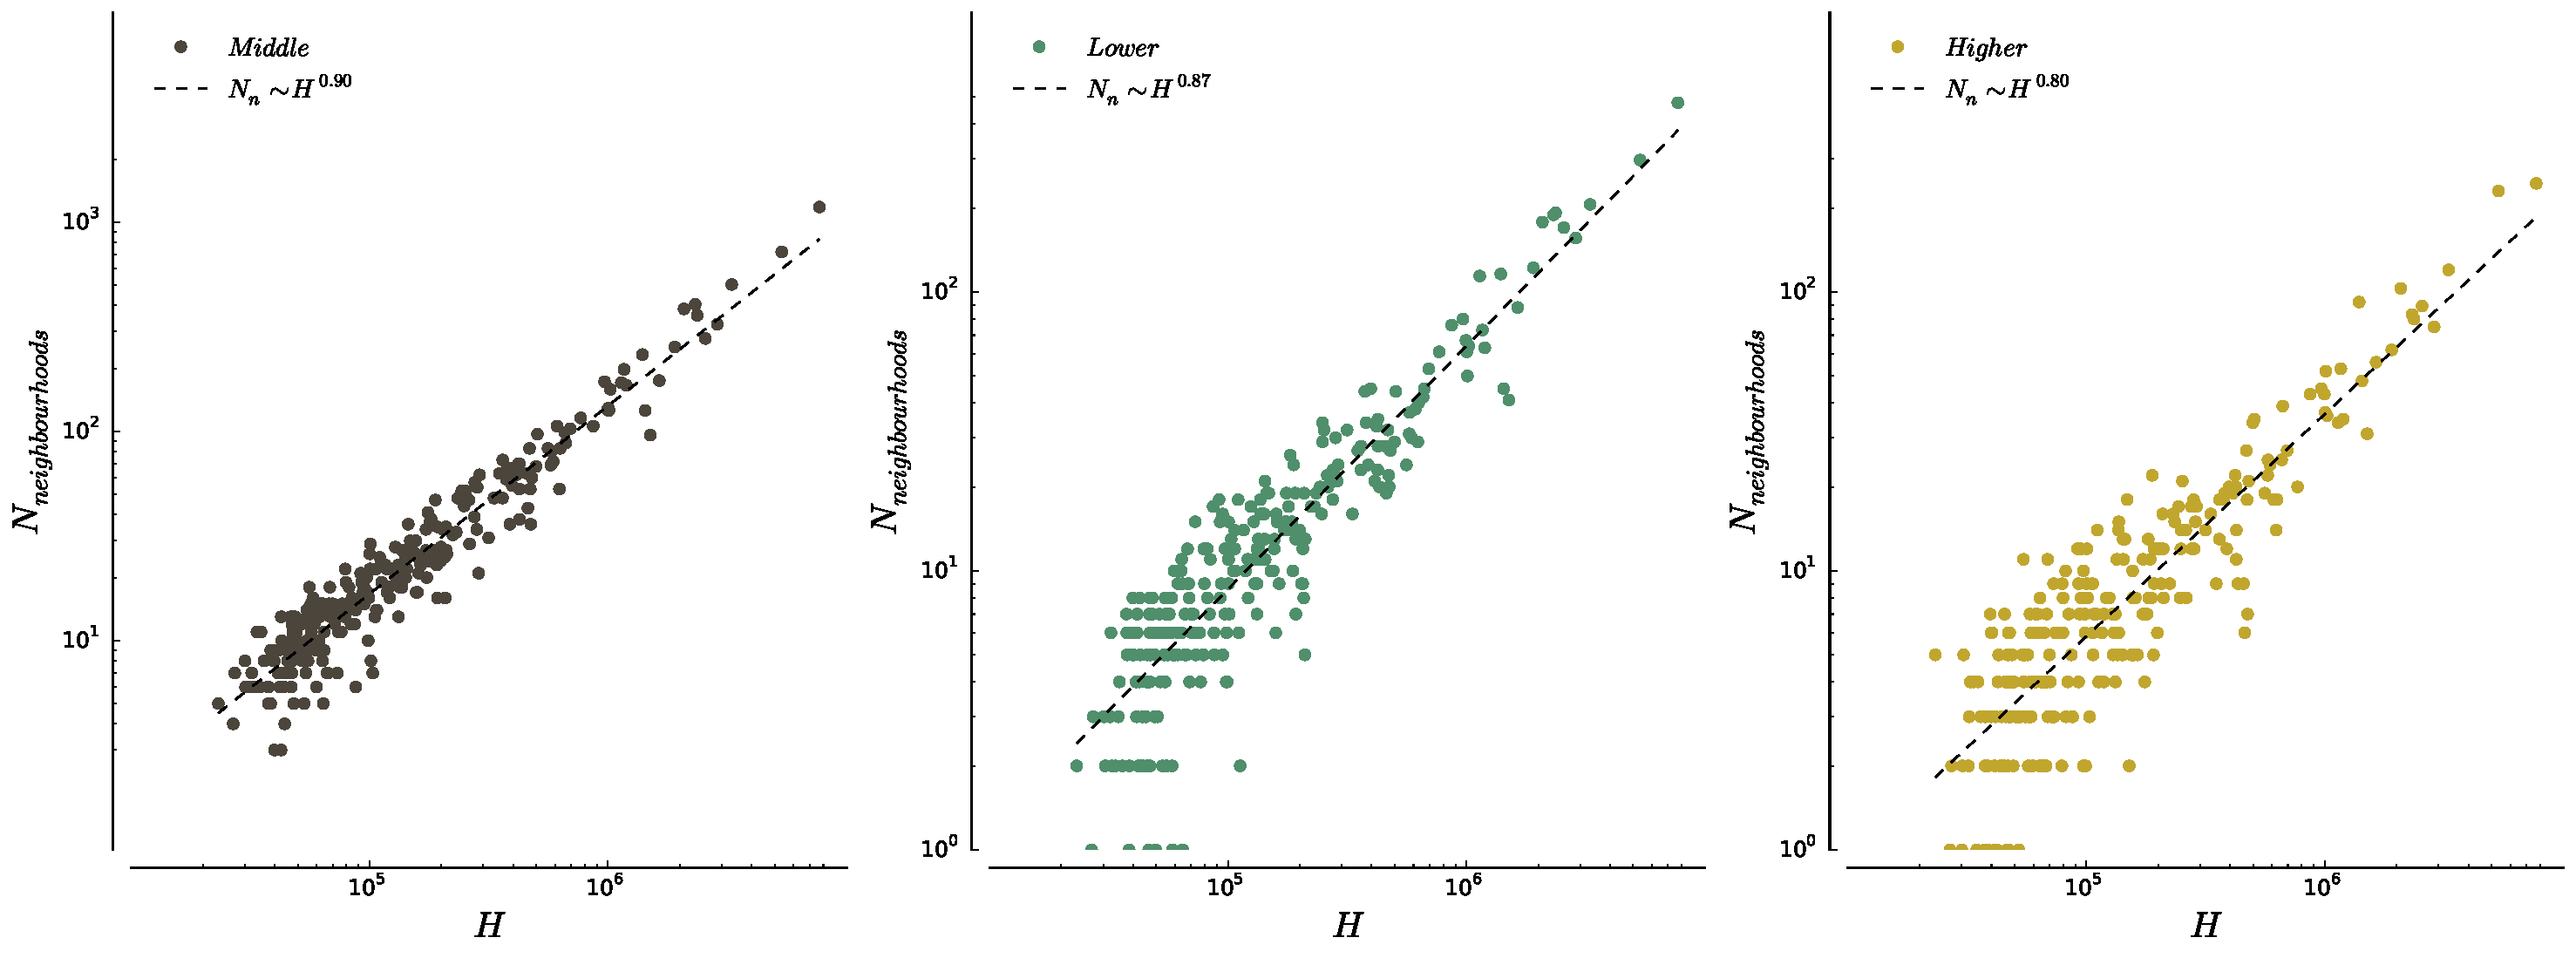
\includegraphics[width=\textwidth]{gfx/chapter-segregation/figure7.pdf}
    \caption{Number of neighbourhoods for the three different classes as a
    function of the size of the city. These plots in loglog show that
    we have a behavior consistent with a power law with exponent less
    than one (and with different value for each class), with $R^2$ values that
    range between $0.88$ (higher-income) and $0.96$ (middle-income). Combined with the linear
    increase of the number of over-represented units with the number of
    households (see SI Appendix),
this sub-linear increase in the number of neighbourhoods shows the tendency of
classes to cluster more as cities get larger.\label{fig:number_clusters_class}}
\end{figure}

\begin{figure}
    \centering
    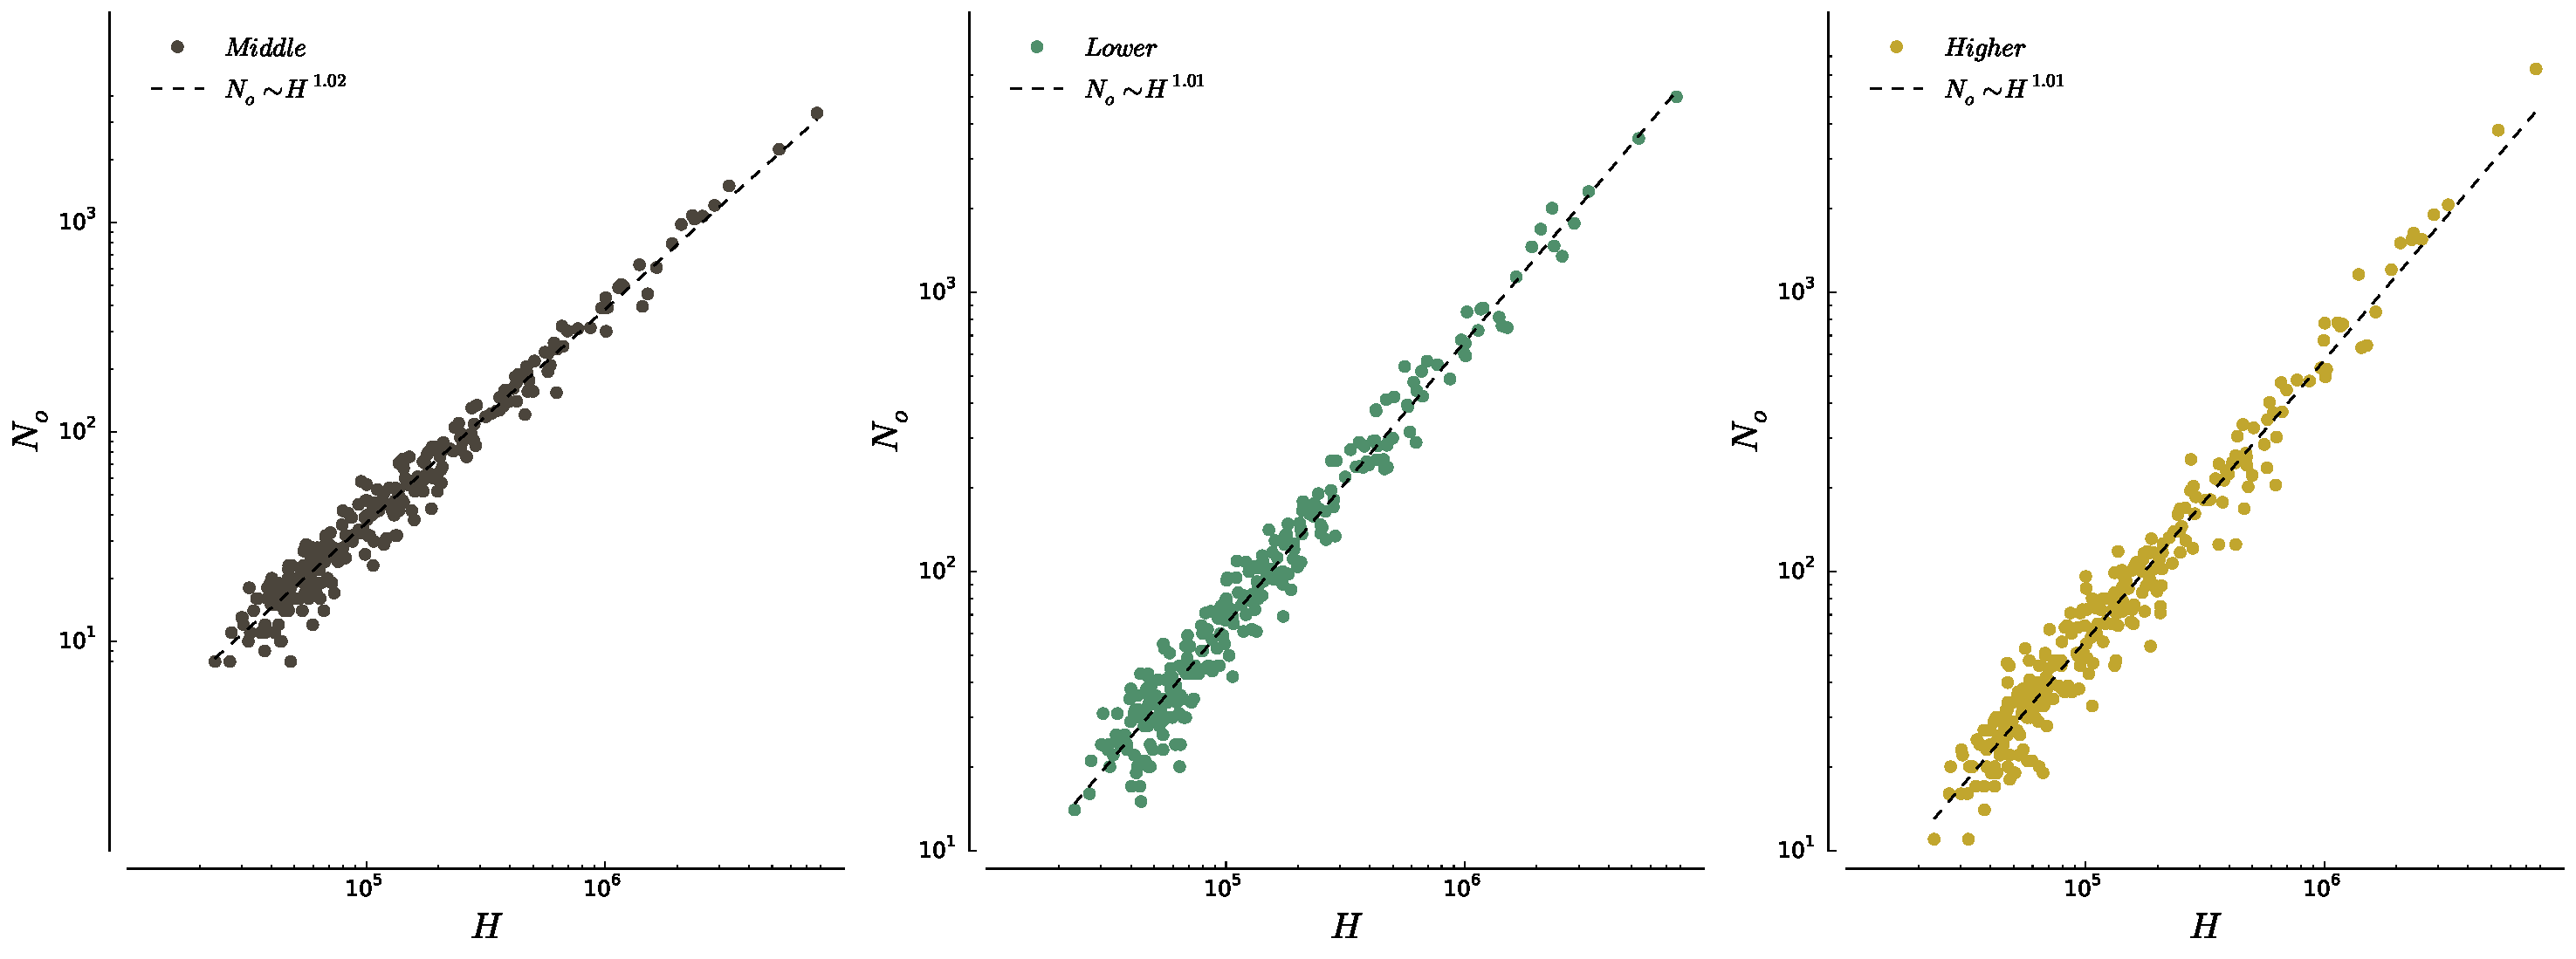
\includegraphics[width=\textwidth]{./gfx/chapter-segregation/number_overrepresented.pdf}
    \caption{Number of areal units where each class is overrepresented as a
    function of the total number of households in the city. The behaviour is
consistent with a linear behaviour in the three cases.
\label{fig:overrepresented}}
\end{figure}


\section{Poor centers, rich suburbs?}
\label{sec:poor_centers_rich_suburbs_}

\begin{figure}
    \centering
    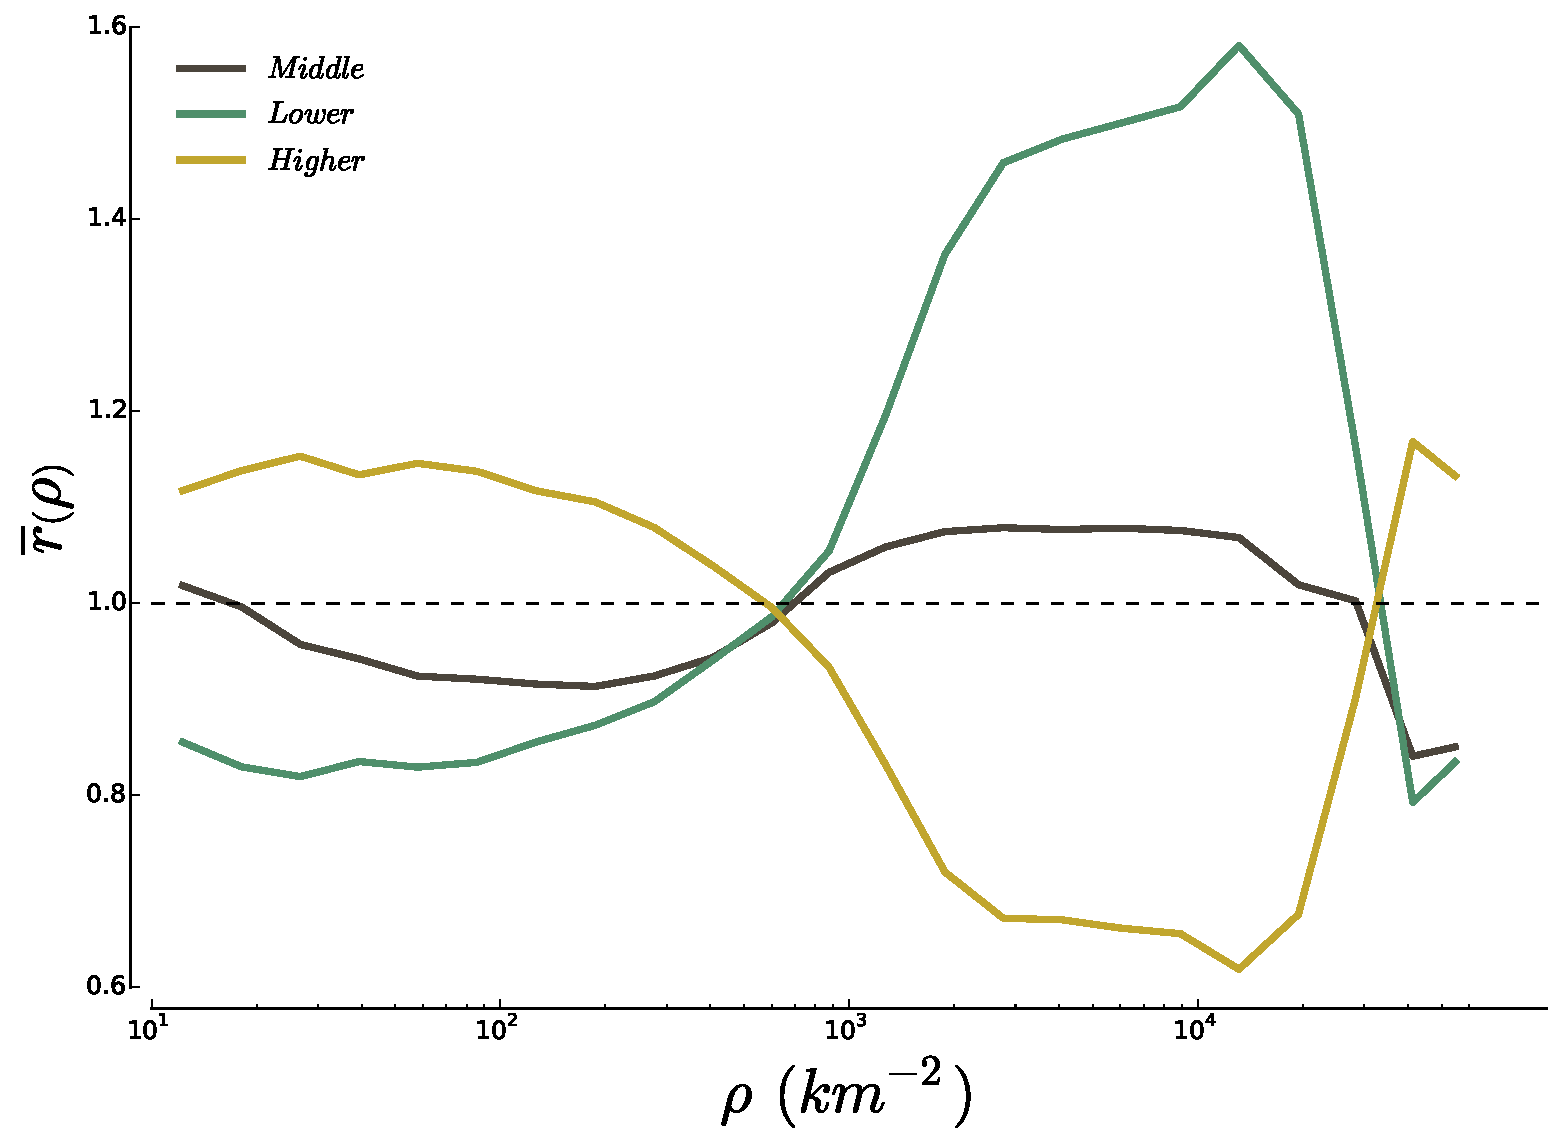
\includegraphics[width=\textwidth]{gfx/chapter-segregation/figure4.pdf}
    \caption{Average representation of the higher-, middle- and
      lower-income classes over the $276$ MSA as a function of the
      local density of households. On average, we find that low-density (the
  suburbs) are rich, while high density regions (the center) are poor,
  confirming empirically on a large dataset a stylized facts that had previously
  emerged from local studies. Interestingly, we also
  find that  very large density areas ($\rho>20,000/km^2$) are rich on average,
  suggesting that density may be one relevant factor in explaining the
  differences between neighbourhoods~\cite{Jacobs:1961}.
  \label{fig:high_low_densities}} 
  \end{figure}

\section{A new measure of segregation}
\label{sec:a_new_measure_of_segregation}


\begin{figure}
    \centering
    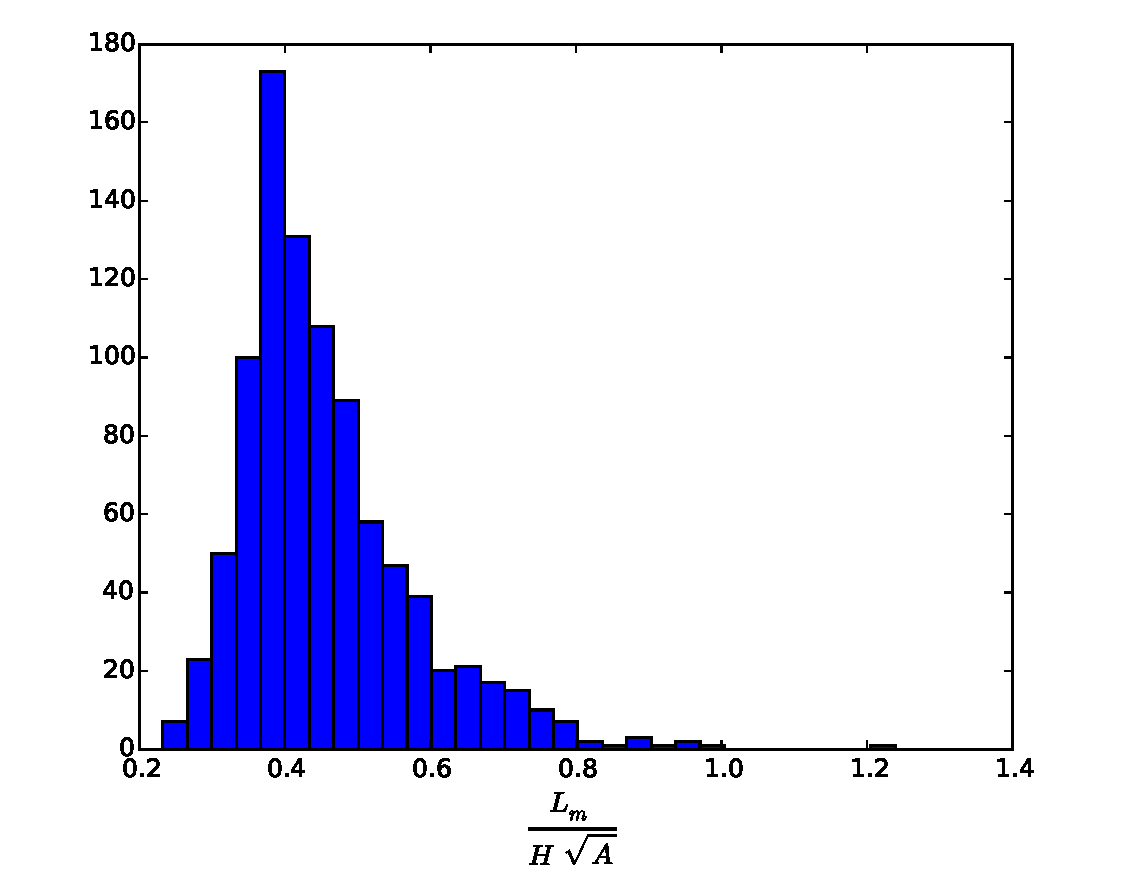
\includegraphics[width=0.75\textwidth]{gfx/chapter-segregation/index_distribution.pdf}
    \caption{Distribution of $e = \frac{L_m}{H\,\sqrt{A}}$ for one realisation
    of the null model for the $\sim 900$ CBSAs in the US. The measure nicely
spans the range $\left[ 0.2, 1 \right]$ with a single town above one (understand
why). \label{fig:label_fig}}
\end{figure}


\begin{figure}
    \centering
    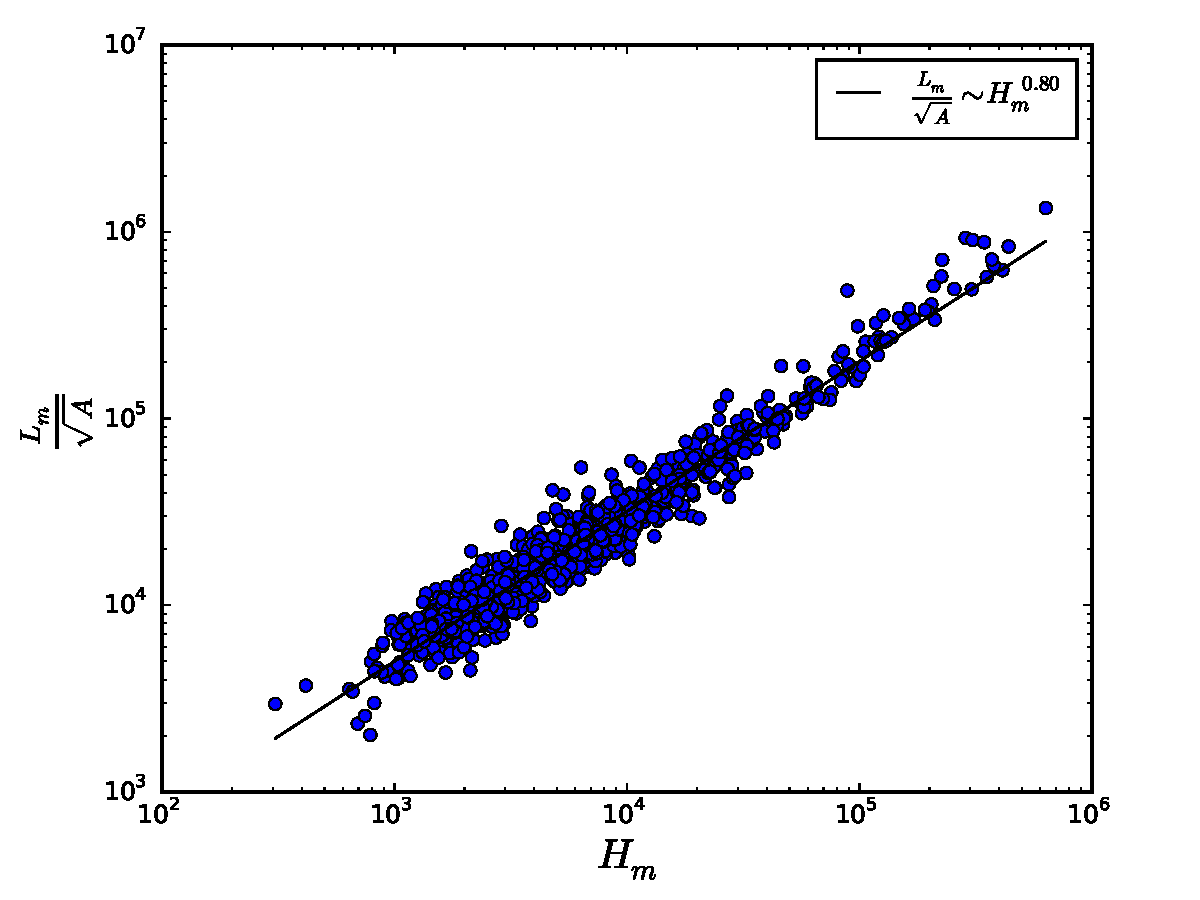
\includegraphics[width=0.75\textwidth]{gfx/chapter-segregation/distance_scaling.pdf}
    \caption{Distance that households would have to move as a
    function of the number of households that would have to move, normalised by
    the typical size of the city they're in. The sublinear
scaling indicates that as cities get larger, households would have to travel a
shorter distance.\label{fig:label_fig}}
\end{figure}


\begin{figure}
    \centering
    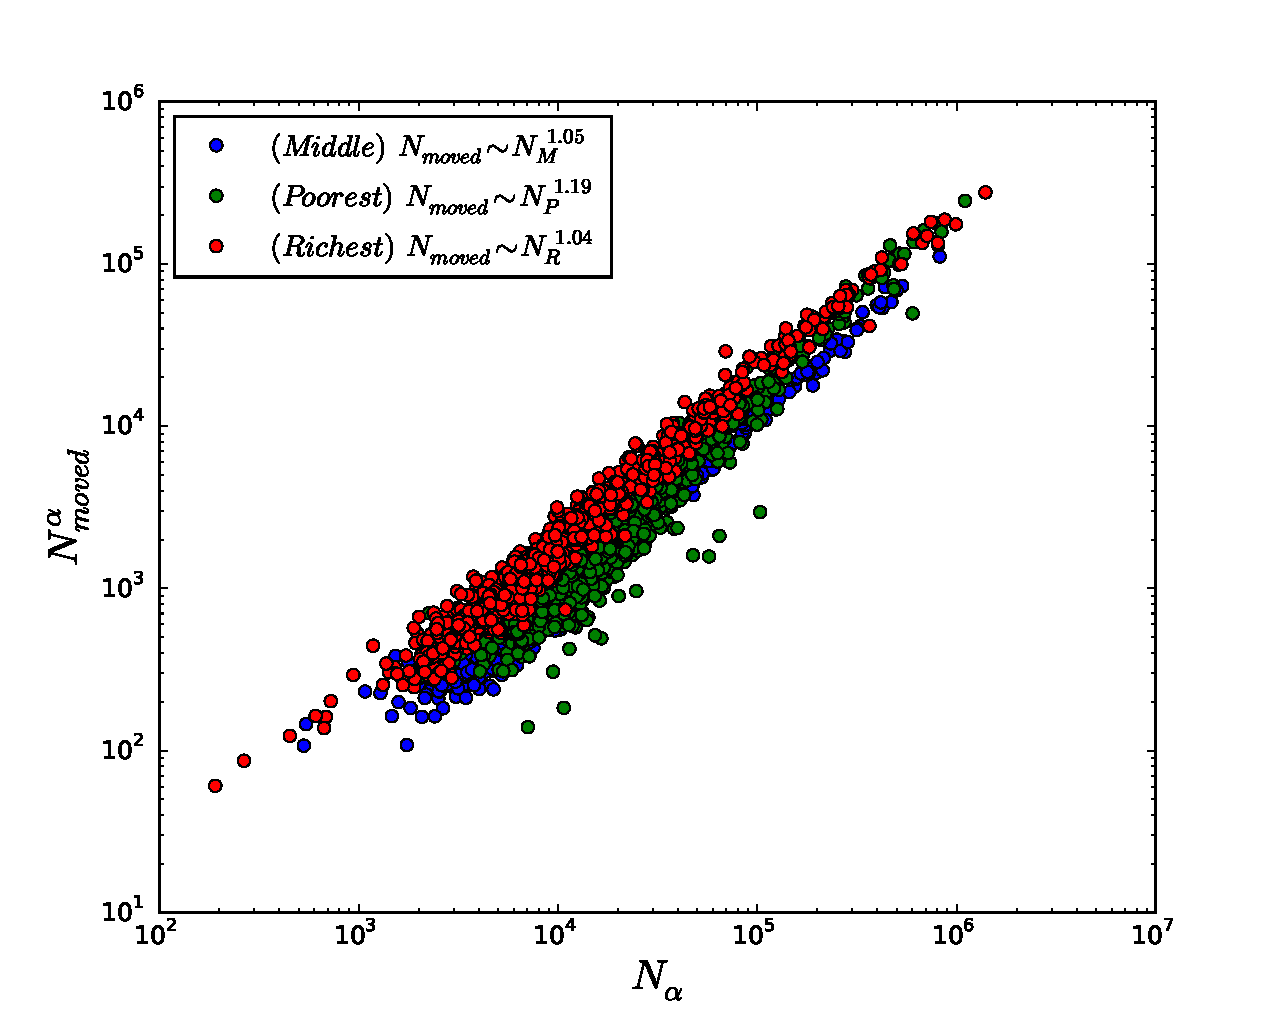
\includegraphics[width=0.75\textwidth]{gfx/chapter-segregation/moved_scaling}
    \caption{Number of people that would have to move to get to the quilibrium
    state as a function of the total population. \label{fig:label_fig}}
\end{figure}


\begin{equation}
    U_\alpha = \frac{1}{2} \sum_{t=1}^T \left| n_\alpha(t) -
    N_\alpha\,\frac{n(t)}{N}\right|
\end{equation}

\begin{equation}
    e = \frac{L_\alpha}{N_\alpha\,D}
\end{equation}

where $L_\alpha$ is the total distance that individuals belonging to the class
$\alpha$ should travel when relocating to obtain a uniform city.
